\documentclass[12pt]{article}
\usepackage[a4paper, top=0.8in, bottom=0.7in, left=0.8in, right=0.8in]{geometry}
\usepackage{amsmath}
\usepackage{amsfonts}
\usepackage{latexsym}
\usepackage{graphicx}
\usepackage{fancyhdr}
\usepackage{enumitem}
\usepackage{setspace}
\usepackage{tcolorbox}
\usepackage{tikz}
\usepackage[defaultfam,tabular,lining]{montserrat} % Font settings for Montserrat

% ChatGPT Directions:
% ----------------------------------------------------------------------
% This template is designed for creating guided lessons that align strictly with specific standards.
% Key points to ensure proper usage:
% 
% 1. **Key Concepts and Vocabulary**:
%    - Include only the concepts necessary for meeting the standards.
%    - Each Key Concept section must align explicitly with the standards being addressed.
%    - If unrelated standards are introduced (e.g., introducing new operations or properties),
%      create additional Key Concept sections labeled ""Part 2,"" ""Part 3,"" etc.
% 2. **Examples**:
%    - Provide concrete worked examples to illustrate the Key Concepts.
%    - These should directly tie back to the Key Concepts presented earlier.
% 3. **Guided Practice**:
%    - Problems should reinforce Key Concepts and Examples.
%    - Allow for ample spacing between problems to give students room for work.
% 4. **Additional Notes**:
%    - Use this section for helpful but non-essential concepts, strategies, or teacher notes.
%    - Examples: Fact families, properties of operations, or alternative explanations.
% 5. **Independent Practice**:
%    - Provide problems for students to practice Key Concepts individually.
% 6. **Exit Ticket**:
%    - Include a reflective or assessment-based question to evaluate student understanding.
% ----------------------------------------------------------------------

\setlength{\parindent}{0pt}
\pagestyle{fancy}

\setlength{\headheight}{27.11148pt}
\addtolength{\topmargin}{-15.11148pt}

\fancyhf{}
%\fancyhead[L]{\textbf{Standard(s): 3.NF.A.1}}
\fancyhead[R]{\includegraphics[width=0.8cm]{Round Logo.png}} % Placeholder for logo
\fancyfoot[C]{\footnotesize \textcopyright Study Smart Tutors}

\sloppy

\title{}
\date{}
\hyphenpenalty=10000
\exhyphenpenalty=10000

\begin{document}

\subsection*{Instructor Version: Guided Lesson on Understanding Fractions as Parts of a Whole}
\onehalfspacing

% Learning Objective Box
\begin{tcolorbox}[colframe=black!40, colback=gray!5, 
coltitle=black, colbacktitle=black!20, fonttitle=\bfseries\Large, 
title=Learning Objective, halign title=center, left=5pt, right=5pt, top=5pt, bottom=15pt]
\textbf{Objective:} Understand fractions as parts of a whole and represent them on a number line.
\end{tcolorbox}

% Instructor Note
\textcolor{blue}{\textbf{Instructor Note:} Use this objective to frame the lesson. Highlight the connection between fractions and real-world applications, like sharing or dividing objects.}

\vspace{1em}

% Key Concepts and Vocabulary
\begin{tcolorbox}[colframe=black!60, colback=white, 
coltitle=black, colbacktitle=black!15, fonttitle=\bfseries\Large, 
title=Key Concepts and Vocabulary, halign title=center, left=10pt, right=10pt, top=10pt, bottom=15pt]
\textbf{Key Concepts:}
\begin{itemize}
    \item \textbf{Fraction as Part of a Whole:} A fraction represents one or more equal parts of a whole. For example, \( \frac{1}{4} \) represents one part out of four equal parts.
    \item \textbf{Number Line Representation:} Fractions also represent numbers on a number line between 0 and 1. 
    \item \textbf{Numerator and Denominator:}
    \begin{itemize}
        \item \textbf{Numerator:} The top number shows how many parts are taken.
        \item \textbf{Denominator:} The bottom number shows the total number of equal parts.
    \end{itemize}
    \item \textbf{Simplest Form:} A fraction is in its simplest form when the numerator and denominator share no common factors other than 1.
    \item \textbf{Equivalence:} Fractions like \( \frac{2}{4} \) and \( \frac{1}{2} \) represent the same part of a whole.
\end{itemize}
\end{tcolorbox}

% Instructor Note
\textcolor{blue}{\textbf{Instructor Note:} Introduce each key concept with concrete examples. Use visuals like fraction strips, pie charts, or number lines to reinforce understanding.}

\vspace{1em}






% Examples
\begin{tcolorbox}[colframe=black!60, colback=white, 
coltitle=black, colbacktitle=black!15, fonttitle=\bfseries\Large, 
title=Examples with Solutions, halign title=center, left=10pt, right=10pt, top=10pt, bottom=15pt]
\textbf{Example 1: Fraction as a Part of a Whole}
\begin{itemize}
    \item Problem: A pizza is divided into 8 equal slices. If you eat 3 slices, what fraction of the pizza have you eaten?


 \item Visual:
    \begin{center}
        \begin{tikzpicture}
            \fill[gray!30] (0,0) -- (90:1.5) arc[start angle=90, end angle=225, radius=1.5] -- cycle; % Highlight 3/8
            \draw (0,0) circle(1.5);
            \foreach \angle in {0,45,...,315} {
                \draw (0,0) -- (\angle:1.5);
            }
        \end{tikzpicture}
    \end{center}


    \item \textcolor{red}{Solution: You have eaten \( \frac{3}{8} \) of the pizza.}
    \item \textcolor{blue}{\textbf{Instructor Note:} Emphasize the importance of equal parts when discussing fractions. Ask students to think about how many slices are left.}
\end{itemize}




\textbf{Example 2: Representing Fractions on a Number Line}


\begin{itemize}
    \item Problem: Divide the segment from 0 to 1 into 4 equal parts and mark \( \frac{3}{4} \) on the number line.
    \item Visual:
    \begin{center}
        \begin{tikzpicture}[scale=3]
            \draw[thick] (0,0) -- (1,0);
            \foreach \x in {0,0.25,0.5,0.75,1} {
                \draw[thick] (\x,0.05) -- (\x,-0.05);
            }
            \node at (0,-0.15) {\( 0 \)};
            \node at (1,-0.15) {\( 1 \)};
            \node at (0.25,-0.15) {\( \frac{1}{4} \)};
            \node at (0.5,-0.15) {\( \frac{1}{2} \)};
            \node at (0.75,-0.15) {\( \frac{3}{4} \)};
            \fill[red] (0.75,0) circle(0.02); % Mark 3/4
        \end{tikzpicture}
    \end{center}
    \item \textcolor{red}{Solution: Divide the segment from 0 to 1 into 4 equal parts. Count 3 parts starting from 0 and mark \( \frac{3}{4} \).}

    \item \textcolor{blue}{\textbf{Instructor Note:} Use a visual number line to explain the problem step-by-step.}
\end{itemize}



\textbf{Example 3: Equivalence of Fractions}
\begin{itemize}
    \item Problem: Show that \( \dfrac{2}{5} \) and \( \dfrac{4}{10} \) are equivalent.
    \item \textcolor{red}{Solution: Multiply the numerator and denominator of \( \dfrac{2}{5} \) by 2: \( \dfrac{2\times 2}{5 \times 2} = \dfrac{4}{10} \).}
    \item \textcolor{blue}{\textbf{Instructor Note:} It is key that you emphasize that multiplying both the numerator and the denominator by 2 does not change the value of the number because $\dfrac{2}{2} = 1$ and $\dfrac{2}{5} \times 1 = \dfrac{2}{5} $}
  
\end{itemize}








\end{tcolorbox}

\vspace{1em}




% Examples Continued
\begin{tcolorbox}[colframe=black!60, colback=white, 
coltitle=black, colbacktitle=black!15, fonttitle=\bfseries\Large, 
title=Examples with Solutions (Continued), halign title=center, left=10pt, right=10pt, top=10pt, bottom=15pt]



\textbf{Example 4: Simplifying Fractions}
\begin{itemize}
    \item Problem: Simplify \( \frac{6}{8} \).

    \item \textcolor{red}{Solution: Divide the numerator and denominator by their greatest common factor (2). \( \dfrac{6\div2}{8\div2} = \dfrac{3}{4} \). \\ Or using Prime Factorization:  \(\dfrac{6}{8} = \dfrac{3\times 2}{4 \times 2} = \dfrac{3}{4} \) }

\item Visual:
    \begin{center}
        \begin{tikzpicture}
            % Left Pie Chart (6/8)
            \fill[gray!30] (0,0) -- (90:1) arc[start angle=90, end angle=360, radius=1] -- cycle; 
            \draw (0,0) circle(1);
            \foreach \angle in {0,45,...,315} {
                \draw (0,0) -- (\angle:1);
            }
            \node at (0,-1.3) {\( \frac{6}{8} \)};
            % Right Pie Chart (3/4)
            \begin{scope}[xshift=3cm]
                \fill[gray!30] (0,0) -- (90:1) arc[start angle=90, end angle=360, radius=1] -- cycle; 
                \draw (0,0) circle(1);
                \foreach \angle in {0,90,...,270} {
                    \draw (0,0) -- (\angle:1);
                }
                \node at (0,-1.3) {\( \frac{3}{4} \)};
            \end{scope}
        \end{tikzpicture}
    \end{center}

    
    \item \textcolor{blue}{\textbf{Instructor Note:} Discuss how simplifying fractions makes them easier to compare.
    It is key that you emphasize that dividing both the numerator and the denominator by 2 does not change the value of the number because $\dfrac{2}{2} = 1$ and $\dfrac{2}{5} \div 1 = \dfrac{2}{5}$}
      \item \textcolor{blue}{\textbf{Instructor Note:} For students who are having trouble simplifying fractions, consider using the fact that every whole number has a unique prime factorization. Write the prime factorizations of the numerator and denominator to help simplify.}
    
\end{itemize}
\end{tcolorbox}



% Guided Practice with Solutions: Problem 1
\begin{tcolorbox}[colframe=black!60, colback=white, 
coltitle=black, colbacktitle=black!15, fonttitle=\bfseries\Large, 
title=Guided Practice with Solutions (Problem 1), halign title=center, left=10pt, right=10pt, top=10pt, bottom=5pt]

\textbf{Problem 1:} A cake is divided into 6 equal parts. If you eat 2 parts, what fraction of the cake have you eaten? Represent this fraction on a number line.
\begin{center}
    \begin{tikzpicture}[scale=6]
        \draw[thick] (0,0) -- (1,0);
        \foreach \x in {0,0.1667,0.3333,0.5,0.6667,0.8333,1} {
            \draw[thick] (\x,0.05) -- (\x,-0.05);
        }
        \node at (0,-0.15) {\( 0 \)};
        \node at (1,-0.15) {\( 1 \)};
        \foreach \x/\label in {0.1667/\( \frac{1}{6} \), 0.3333/\( \frac{2}{6} \), 0.5/\( \frac{3}{6} \), 0.6667/\( \frac{4}{6} \), 0.8333/\( \frac{5}{6} \)} {
            \node at (\x,-0.15) {\label};
        }
    \end{tikzpicture}
\end{center}
\begin{itemize}
    \item \textcolor{red}{Solution: The fraction of the cake eaten is \( \frac{2}{6} \), which simplifies to \( \frac{1}{3} \). On the number line, \( \frac{2}{6} \) corresponds to the second division from 0.}
    \item \textcolor{blue}{\textbf{Instructor Note:} Highlight that simplification is important for clarity. Show students how to divide the numerator and denominator by their greatest common factor.}
\end{itemize}

\end{tcolorbox}

% Guided Practice with Solutions: Problems 2–6
\begin{tcolorbox}[colframe=black!60, colback=white, 
coltitle=black, colbacktitle=black!15, fonttitle=\bfseries\Large, 
title=Guided Practice with Solutions (Problems 2–6), halign title=center, left=10pt, right=10pt, top=10pt, bottom=15pt]

\textbf{Problem 2:} Divide the segment from 0 to 1 into 5 equal parts. Mark \( \frac{2}{5} \) and \( \frac{4}{5} \) on the number line.
\begin{center}
    \begin{tikzpicture}[scale=5]
        \draw[thick] (0,0) -- (1,0);
        \foreach \x in {0,0.2,0.4,0.6,0.8,1} {
            \draw[thick] (\x,0.05) -- (\x,-0.05);
        }
        \node at (0,-0.15) {\( 0 \)};
        \node at (1,-0.15) {\( 1 \)};
        \foreach \x/\label in {0.2/\( \frac{1}{5} \), 0.4/\( \frac{2}{5} \), 0.6/\( \frac{3}{5} \), 0.8/\( \frac{4}{5} \)} {
            \node at (\x,-0.15) {\label};
        }
    \end{tikzpicture}
\end{center}
\begin{itemize}
    \item \textcolor{red}{Solution: \( \frac{2}{5} \) is marked at the second division, and \( \frac{4}{5} \) is marked at the fourth division on the number line.}
    \item \textcolor{blue}{\textbf{Instructor Note:} Explain the importance of equally dividing the number line. Relate the numerator to steps from 0 and the denominator to the total number of parts.}
\end{itemize}

\vspace{1em}

\textbf{Problem 3:} A pie is divided into 4 equal parts. If you eat 3 parts, what fraction of the pie have you eaten? Represent this on a pie chart.
\begin{center}
    \begin{tikzpicture}[scale=1]
        \fill[gray!30] (0,0) -- (90:1) arc[start angle=90, end angle=360, radius=1] -- cycle; % Highlight 3/4
        \draw (0,0) circle(1);
        \foreach \angle in {0,90,...,270} {
            \draw (0,0) -- (\angle:1);
        }
    \end{tikzpicture}
\end{center}
\begin{itemize}
    \item \textcolor{red}{Solution: The fraction of the pie eaten is \( \frac{3}{4} \). The pie chart highlights 3 out of 4 equal parts.}
    \item \textcolor{blue}{\textbf{Instructor Note:} Use this visual to reinforce the connection between fractions and real-world division of objects. Discuss how \( \frac{3}{4} \) represents both parts of the whole and a numerical value.}
\end{itemize}

\vspace{1em}

\textbf{Problem 4:} Divide a segment from 0 to 2 into 8 equal parts. Mark \( \frac{3}{8} \) and \( \frac{7}{8} \) on the number line.
\begin{center}
    \begin{tikzpicture}[scale=4]
        \draw[thick] (0,0) -- (2,0);
        \foreach \x in {0,0.25,...,2} {
            \draw[thick] (\x,0.05) -- (\x,-0.05);
        }
        \node at (0,-0.15) {\( 0 \)};
        \node at (2,-0.15) {\( 2 \)};
        \foreach \x/\label in {0.25/\( \frac{1}{8} \), 0.5/\( \frac{2}{8} \), 0.75/\( \frac{3}{8} \), 
                              1/\( \frac{4}{8} \), 1.25/\( \frac{5}{8} \), 1.5/\( \frac{6}{8} \), 
                              1.75/\( \frac{7}{8} \)} {
            \node at (\x,-0.15) {\label};
        }
    \end{tikzpicture}
\end{center}
\begin{itemize}
    \item \textcolor{red}{Solution: \( \frac{3}{8} \) is at the third division, and \( \frac{7}{8} \) is at the seventh division.}
    \item \textcolor{blue}{\textbf{Instructor Note:} Emphasize that the denominator represents total parts across the entire segment, while the numerator identifies the count starting from 0.}
\end{itemize}

\vspace{1em}


\end{tcolorbox}

\vspace{1em}

% Independent Practice
\begin{tcolorbox}[colframe=black!60, colback=white, 
coltitle=black, colbacktitle=black!15, fonttitle=\bfseries\Large, 
title=Independent Practice, halign title=center, left=10pt, right=10pt, top=10pt, bottom=15pt]

\textbf{Problem 1:} A chocolate bar is divided into 12 equal pieces. If 4 pieces are eaten, what fraction is left? Represent this fraction visually with a bar diagram.
\begin{center}
    \begin{tikzpicture}[scale=1]
        \foreach \x in {0,1,2,3,4,5,6,7,8,9,10,11} {
            \fill[gray!30] (\x,0) rectangle ++(1,1); % All pieces
        }
        \foreach \x in {0,1,2,3} {
            \fill[white] (\x,0) rectangle ++(1,1); % Eaten pieces
        }
        \draw[step=1cm] (0,0) grid (12,1);
    \end{tikzpicture}
\end{center}

\begin{itemize}
    \item \textcolor{red}{Solution: 4 pieces are eaten, leaving \( \frac{8}{12} \) pieces, which simplifies to \( \frac{2}{3} \).}
    \item \textcolor{blue}{\textbf{Instructor Note:} Discuss how subtraction is used to find the remaining fraction and reinforce the importance of simplification.}
\end{itemize}

\vspace{1em}

\textbf{Problem 2:} A rope is divided into 10 equal parts. If you use 6 parts for tying, what fraction of the rope is used? Represent this on a bar diagram.
\begin{center}
    \begin{tikzpicture}[scale=1]
        \foreach \x in {0,1,2,3,4,5,6,7,8,9} {
            \fill[gray!30] (\x,0) rectangle ++(1,1); % All parts
        }
        \foreach \x in {0,1,2,3,4,5} {
            \fill[black!50] (\x,0) rectangle ++(1,1); % Used parts
        }
        \draw[step=1cm] (0,0) grid (10,1);
    \end{tikzpicture}
\end{center}

\begin{itemize}
    \item \textcolor{red}{Solution: \( \frac{6}{10} \) parts are used, which simplifies to \( \frac{3}{5} \).}
    \item \textcolor{blue}{\textbf{Instructor Note:} Use this diagram to emphasize the proportion of the rope used versus what remains. Encourage students to simplify the fraction for clarity.}
\end{itemize}

\vspace{1em}

\textbf{Problem 3:} A water tank is divided into 8 equal sections. If \( \frac{5}{8} \) of the tank is filled, how many sections remain empty? Represent this visually using a bar diagram.
\begin{center}
    \begin{tikzpicture}[scale=1]
        \foreach \x in {0,1,2,3,4,5,6,7} {
            \fill[gray!30] (\x,0) rectangle ++(1,1); % All sections
        }
        \foreach \x in {0,1,2,3,4} {
            \fill[blue!50] (\x,0) rectangle ++(1,1); % Filled sections
        }
        \foreach \x in {5,6,7} {
            \fill[white] (\x,0) rectangle ++(1,1); % Empty sections
        }
        \draw[step=1cm] (0,0) grid (8,1);
    \end{tikzpicture}
\end{center}

\begin{itemize}
    \item \textcolor{red}{Solution: If \( \frac{5}{8} \) of the tank is filled, \( \frac{3}{8} \) remains empty. This corresponds to 3 sections out of the total 8 sections.}
    \item \textcolor{blue}{\textbf{Instructor Note:} Discuss the relationship between the fraction filled and the fraction remaining. Reinforce how subtraction can help find the missing part of the whole.}
\end{itemize}

\end{tcolorbox}




\vspace{1em}
% Independent Practice Continued
\begin{tcolorbox}[colframe=black!60, colback=white, 
coltitle=black, colbacktitle=black!15, fonttitle=\bfseries\Large, 
title=Independent Practice Continued, halign title=center, left=10pt, right=10pt, top=10pt, bottom=15pt]
\textbf{Problem 4:} A rectangle is divided into 4 equal parts horizontally. If you shade \( \frac{3}{4} \), how many parts are shaded, and how many are unshaded? Represent this visually.
\begin{center}
    \begin{tikzpicture}[scale=1]
        \foreach \y in {0,1,2,3} {
            \fill[gray!30] (0,-\y) rectangle ++(4,-1); % All parts
        }
        \foreach \y in {0,1,2} {
            \fill[blue!50] (0,-\y) rectangle ++(4,-1); % Shaded parts
        }
        \draw[step=1cm] (0,-4) grid (4,0);
    \end{tikzpicture}
\end{center}

\begin{itemize}
    \item \textcolor{red}{Solution: \( \frac{3}{4} \) is shaded, representing 3 parts. \( \frac{1}{4} \) remains unshaded, corresponding to 1 part.}
    \item \textcolor{blue}{\textbf{Instructor Note:} Discuss how shading and unshading can represent fractions visually. Highlight the relationship between the total and its parts.}
\end{itemize}

\end{tcolorbox}


\vspace{3 cm}

% Exit Ticket with Solution
\begin{tcolorbox}[colframe=black!60, colback=white, 
coltitle=black, colbacktitle=black!15, fonttitle=\bfseries\Large, 
title=Exit Ticket with Solutions, halign title=center, left=10pt, right=10pt, top=10pt, bottom=15pt]
\textbf{Question 1:} How can fractions be represented on a number line? Provide an example.
\begin{itemize}
    \item \textcolor{red}{Solution: Fractions are represented by dividing the segment between 0 and 1 into equal parts. For example, \( \frac{2}{5} \) is represented by dividing the segment into 5 parts and marking the second point.}
    \item \textcolor{blue}{\textbf{Instructor Note:} Encourage students to practice drawing number lines independently.}
\end{itemize}
\end{tcolorbox}

\end{document}
